\documentclass[a4paper]{exam}

\usepackage{geometry}
\usepackage{graphicx}
\usepackage{hyperref}
\usepackage{titling}

\printanswers

\title{Weekly Challenge 03: Growth of Functions\\CS 412 Algorithms: Design and Analysis}
\author{team-name}  % <==== replace with your team name for grading
\date{Habib University | Spring 2023}

\runningheader{CS 412: Algorithms}{WC03: Growth of Functions}{\theauthor}
\runningheadrule
\runningfootrule
\runningfooter{}{Page \thepage\ of \numpages}{}

\qformat{{\large\bf \thequestion. \thequestiontitle}\hfill}
\boxedpoints

\begin{document}
\maketitle

\begin{questions}
  
  \titledquestion{Robot Race}
  
  \begin{figure*}[!h]
    \centering
    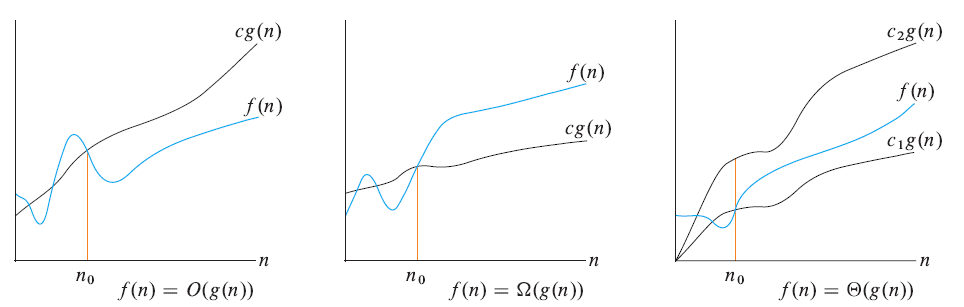
\includegraphics[width=.95\textwidth]{asymptotic}
    
    \caption{Graphical examples of the $O, \Omega$, and $\Theta$ notations \cite{clrs}.}
    \label{fig:notation}
  \end{figure*}
  
  You have designed a robot to compete in a race on a track that is $n$ units long. Your robot can cover $1$ or $2$ units in a single step. At the start of the race, your robot generates all possible sequences of steps to cover the $n$ units and evaluates each sequence according to various parameters---wind condition, battery, competitive advantage, status of the joints, etc.---in order to pick an optimum. We are interested in estimating, $f(n)$, the size of the solution space, i.e. the number of sequences that the robot has to consider, for a given $n$.
  
  \paragraph{Example} The table below shows the possible sequences for some values of $n$ and the resulting value of $f(n)$.
  
  \begin{tabular}{|l|l|l|}
    \hline
    $n$ & Possible sequences& $f(n)$ \\
    \hline\hline
    1 & $\{1\}$ & 1 \\
    4 & $\{1,1,1,1\}$, $\{1,1,2\}$, $\{1,2,1\}$, $\{2,1,1\}$, $\{2,2\}$ & 5 \\
    \hline
  \end{tabular}
  
  \paragraph{Tasks}
  \begin{itemize}
  \item Implement the function, \texttt{num\_sequences}, in the accompanying file, \texttt{test\_sequences.py}, that returns the size of the solution space for a given $n$.
  \item Run \texttt{pytest} locally to check your implementation.
  \item Include in the solution below, a diagram containing a plot of $f(n)$ against $n$ for $n$ in \texttt{range(1,20002, 100)}.
  \item Add to your diagram, plots for $c_1f_1(n)$, $c_2f_2(n)$, $d_1g(n)$ and $d_2g(n)$, where $f(n)=O(f_1(n))=\Omega(f_2(n))=\Theta(g(n))$ and $c_1,c_2,d_1$, and $d_2$ are the corresponding constants.
  \item Make sure that each plot is clearly labeled, or the diagram contains a clearly visible legend.
  \item Make sure that the axis limits are set such that the plots are clearly visible and occupy a large portion of the diagram.
  \item Indicate the expressions/values for  $f_1(n), f_2(n), g(n), c_1,c_2,d_1$, and $d_2$ in your solution below.
  \item Argue below for the values of the constants.
  \item Share your diagram as a comment on the \href{https://web.yammer.com/main/org/habib.edu.pk/threads/eyJfdHlwZSI6IlRocmVhZCIsImlkIjoiMjEwMjY3NTY0NDY3ODE0NCJ9}{WC03 post} in the course group.
  \end{itemize}
  \underline{Tip}: You may consider \href{https://matplotlib.org/stable/tutorials/introductory/pyplot.html}{\texttt{matplotlib}} for plotting purposes.

  
  \begin{thebibliography}{9}
  \bibitem{clrs}
    Thomas H. Cormen, Charles E. Leiserson, Ronald L. Rivest, and Clifford Stein. 2022. \textit{Introduction to Algorithms}, Eighth Edition (8th. ed.). The MIT Press.
  \end{thebibliography}

  \begin{solution}
    
  \end{solution}

\end{questions}

\end{document}
